\chapter{Cross-Checking the Efficiency Estimates of MVA Features}
\label{chap:apdx_mva_xcheck}
\chapquote{Dowerjai, no prowerjai.}{Vladimir Lenin, allegedly.}
In the realm of machine learning, interpretability of trained models has become an important topic and new explanation methods pop up frequently, \eg{}, Refs.~\cite{nnexplain1,nnexplain2,nnexplain3}.
In \gls{hep} applications and in particular in the context of (binary) classification problems where training instances of the labels \textit{signal} and \textit{background} are drawn from separate sources, \ie{}, from \gls{mc} simulated events (signal) and recorded data (background), the question arises to what degree these training data are representative of the real data.
Again, various approaches came up lately to tackle this question
when the training data are not representative of the real data, \eg{}, Refs.~\cite{nnexplain_hep1,nnexplain_hep2}.
In the context of the present analysis, we limit ourself to the study of the fidelity of the classifier responses that we evaluate with \gls{mc} simulated events in order to obtain the efficiencies of our classification.
If certain nuisance parameters would be present, which would help our classifiers to learn to distinguish recorded data from simulated events rather than signal and background signatures (in recorded data), the classifiers, as well as estimated efficiencies would be worthless.

To keep our model verifiable w.r.t.\ the estimated efficiencies without using sophisticated yet complex approaches as proposed in Ref.~\cite{nnexplain_hep1}, we split our classifiers into two disjoint sub-classifiers (\cf{}~Sec.~\ref{sec:LbToDzLz_tightsel}) which can now be verified using a data driven approach.
These two classifiers, the \Lz classifier and the \Lb-\Dz classifier, are applied to recorded \decay{\Lb}{\jpsi\Lz} and \decay{\Lb}{\Dz\proton\pim} candidates which we used previously for estimating the calibration factors (\cf{}~Chap.~\ref{chap:weights}) and the normalization (\cf{}~Chap.~\ref{chap:norm}), respectively.
The rich statistics and the clean data samples allow an efficiency estimation using recorded data, leveraging the direct comparison of these figures with the predictions from simulated events.\footnote{This approach implicitly assumes common fidelity issues of the respective features among the simulated \Lb decays.}

In Sec.~\ref{sec:apdx_mva_xcheck_effest} we outline our strategy for extracting the efficiencies.
We will find a sufficient fidelity of all used classifiers.
The proxy modes also allow an estimation of the fidelity of the \gls{dtf} probability distribution where we witness a large deviation for \gls{DD} tracks.
The deviation, as well as the implication are discussed in Sec.~\ref{sec:apdx_mva_xcheck_pdtf}.

\section{Efficiency Estimation}
\label{sec:apdx_mva_xcheck_effest}
The efficiency $\varepsilon_f$ of a feature $f$ is defined as the ratio
\begin{equation*}
    \varepsilon_f := \frac{n_F}{n_{F \setminus f}} \,,
\end{equation*}
where $n_F$ is the amount of events that are left after requiring the full selection $F$ (see below) and $n_{F \setminus f}$ is the corresponding amount if feature $f$ is left out.
The definition of the full selection $F$ depends on the proxy mode.
Whether or not a feature is included in $F$ of a given proxy mode is listed in Tab.~\ref{tab:apdx_mva_xcheck_effs}, as well as the estimated efficiencies.
If a given feature $f$ is included in $F$, it obeys the selection thresholds of the dedicated \decay{\Lb}{\Dz\Lz} tight selection (\cf{}~Sec.~\ref{sec:LbToDzLz_tightsel}), except for the \gls{dtf} probability of the \decay{\Lb}{\Dz\proton\pim} proxy.
(The performance of the \gls{dtf} probability is discussed separately in Sec.~\ref{sec:apdx_mva_xcheck_pdtf}.)
\begin{table}[htbp]
    \centering
    \caption{Efficiency estimates of the tier~2 features, obtained from recorded data and \gls{mc} simulated events, as well as the corresponding (daughters of the) proxy modes. The efficiencies $\varepsilon_f$ are defined as the ratio of the amounts $n_F$ and $n_{F \setminus f}$, where $n_F$ is the amount of events that are left after requiring features to obey the dedicated \decay{\Lb}{\Dz\Lz} tight selection (if having a counter part in the proxy mode) and $n_{F \setminus f}$ is the corresponding amount if feature $f$ is left out. In the last column we list the residuals of the ratios which are taken as systematic deviations due to an imperfect simulation fidelity. In the bottom row we give the sum in quadrature of these uncertainties.}
    \label{tab:apdx_mva_xcheck_effs}
    \begin{tabular}{ll%
                    S[separate-uncertainty=false,table-format=2.2(2)]%
                    S[separate-uncertainty=false,table-format=2.2(2)]%
                    S[separate-uncertainty=false,table-format=2.2(2)]%
                    S[separate-uncertainty=false,table-format=2.2(2)]%
                    S[separate-uncertainty=false,table-format=2.1(2)]%
                    S[separate-uncertainty=false,table-format=2.1(2)]}
        \toprule
        && \multicolumn{2}{c}{{Rec.\ data [\%]}} & \multicolumn{2}{c}{{\gls{mc} sim. [\%]}} & \multicolumn{2}{c}{{$1 - \text{ratio}$ [\%]}} \\
        Feature & Proxy & \gls{LL} & \gls{DD} & \gls{LL} & \gls{DD} & \gls{LL} & \gls{DD} \\
        \midrule
        \Lz Clf. & \jpsi\Lz & 85.5 \pm 1.3 & 23.4 \pm 0.6 & 85.8 \pm 0.7 & 23.82 \pm 0.19 & 0.4 \pm 1.8 & 1.6 \pm 2.6 \\
        \Lb-\Dz Clf. & \PD\proton\pion & 80.6 \pm 0.7 & 38.8 \pm 0.4 & 78.35 \pm 0.06 & 37.79 \pm 0.05 & -2.9 \pm 0.8 & -2.8 \pm 1.1 \\
        \Gls{dtf} & \jpsi\Lz & 85.4 \pm 1.4 & 59.3 \pm 1.7 & 87.9 \pm 0.7 & 72.6 \pm 0.7 & 2.9 \pm 1.8 & 18.3 \pm 2.5 \\
        \Gls{dtf} & \PD\proton\pion & 94.1 \pm 0.7 & 94.4 \pm 1.1 & 97.96 \pm 0.09 & 97.67 \pm 0.18 & 3.9 \pm 0.8 & 3.3 \pm 1.2 \\
        $\texttt{ProbNNp}(\proton)$ & \jpsi\Lz & 90.5 \pm 1.3 & 81.9 \pm 3.2 & 94.4 \pm 0.8 & 83.7 \pm 0.8 & 4.1 \pm 1.6 & 2 \pm 4 \\
        $\texttt{ProbNNk}(\kaon)$ & \PD\proton\pion & 89.8 \pm 0.7 & 81.2 \pm 1.0 & 91.23 \pm 0.08 & 84.26 \pm 0.15 & 1.8 \pm 0.8 & 3.6 \pm 1.2 \\
        \midrule
        &&&&&& {$7\,\%$} & {$19\,\%$} \\
        \bottomrule
    \end{tabular}
\end{table}
The amounts $n_F$ and $n_{F \setminus f}$ are obtained using the outlined fit approaches in Sec.~\ref{sec:weights_tightsel} and Sec.~\ref{sec:LbToDzppi_yields}.
In order to test the sensitivity of the calibration of recorded \decay{\Lb}{\Dz\proton\pim} data (\cf{}~Sec.~\ref{sec:norm_calibration}) we estimate the efficiency with and without calibration and find deviations below $5\,\%$, \ie{}, our feature selection only depends weakly on resonance structures.
In Fig.~\ref{fig:LbToDzppi_mvaxcheck_hLbM} we show the invariant mass distributions used for extracting the efficiency of the \texttt{ProbNNk} classifier as an example.
Since the efficiency is obtained by taking the ratio of fitted yields, the bias of the fit model as discussed in Sec.~\ref{sec:LbToDzppi_yields} only plays a minor role in the ratio.
In the case of \decay{\Lb}{\jpsi\Lz}, the subset of the dedicated \decay{\Lb}{\Dz\Lz} tight selection, even though not optimized for the proxy mode, suppresses almost all background events as shown in Fig.~\ref{fig:LbToJpsiLz_mvaxcheck_hLbM_allcuts}, again allowing a low-bias extraction of the feature efficiencies.
\begin{figure}[htbp]
    \centering
    \begin{subfigure}{.49\textwidth}
        \centering
        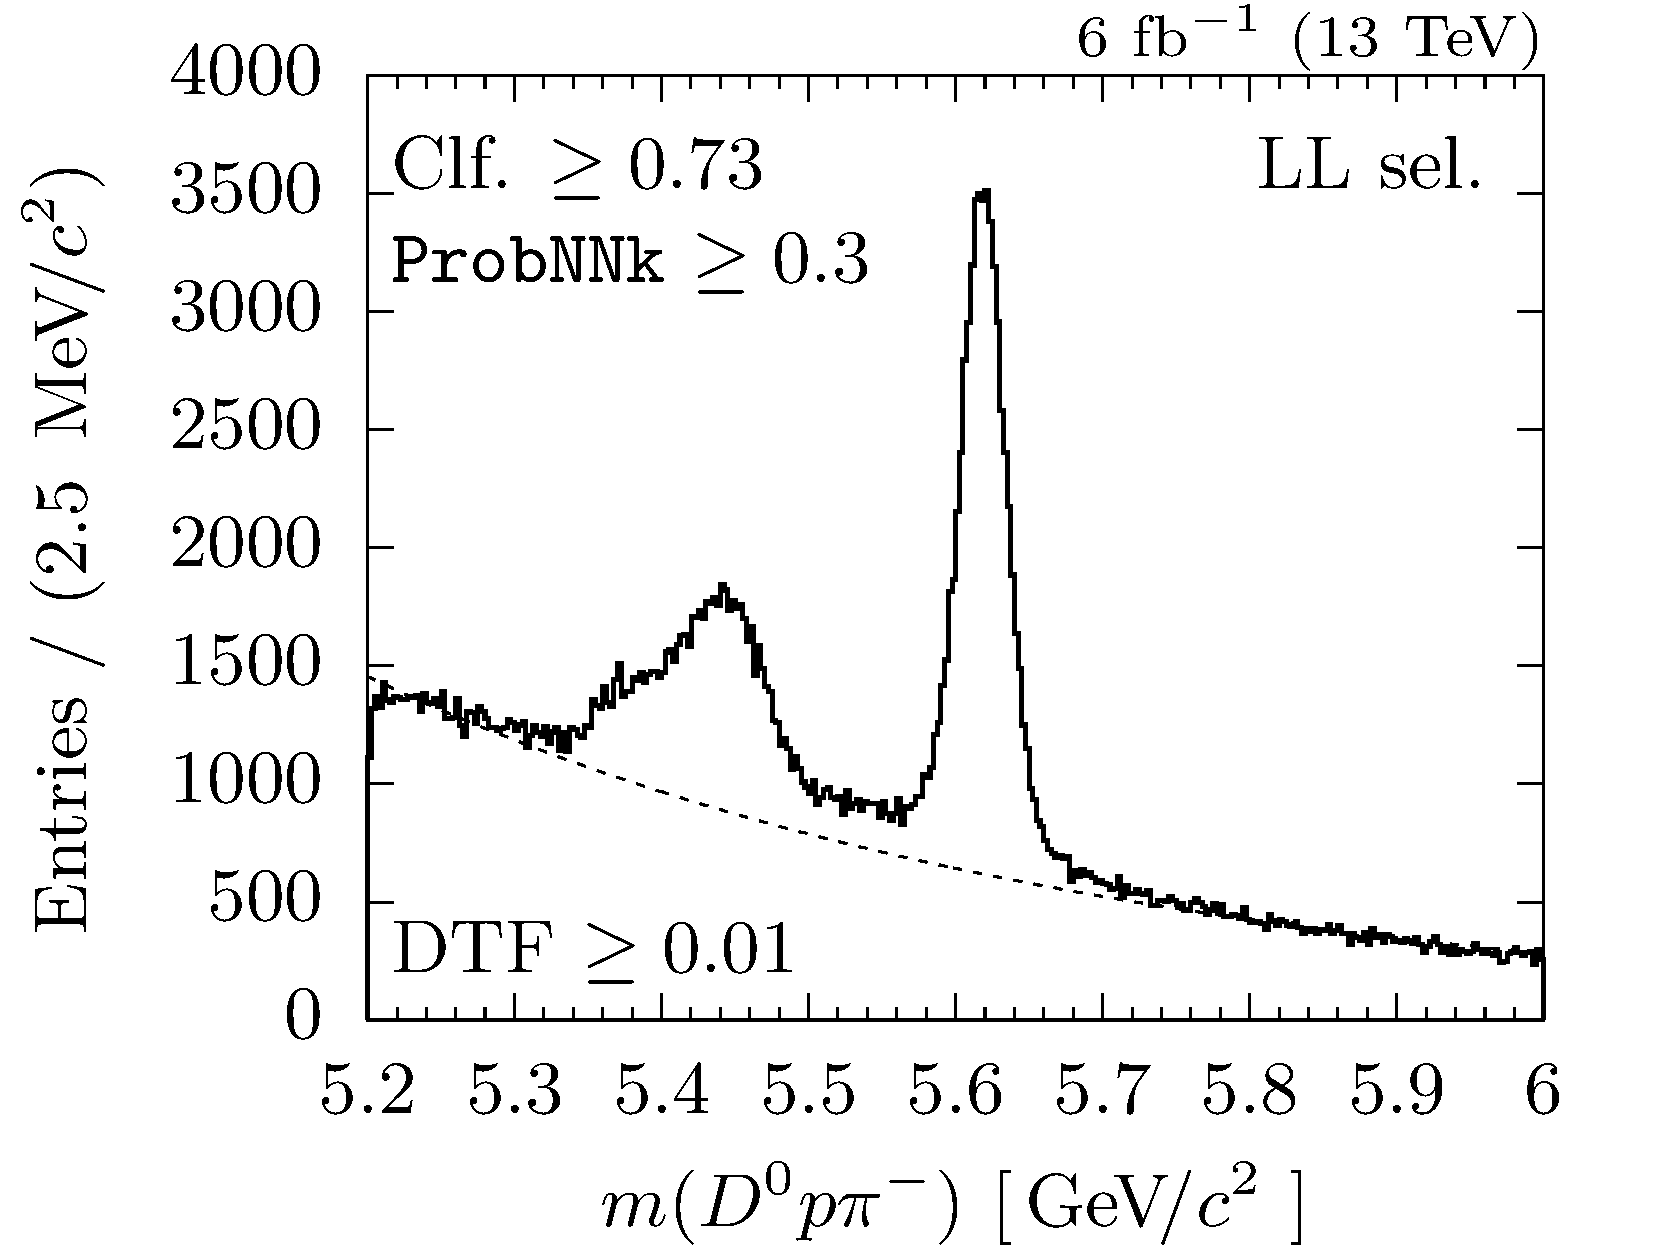
\includegraphics[scale=1.]{Lb2Dzppi_mvaxcheck/hLbM_LL_allcuts.png}
    \end{subfigure}
    \begin{subfigure}{.49\textwidth}
        \centering
        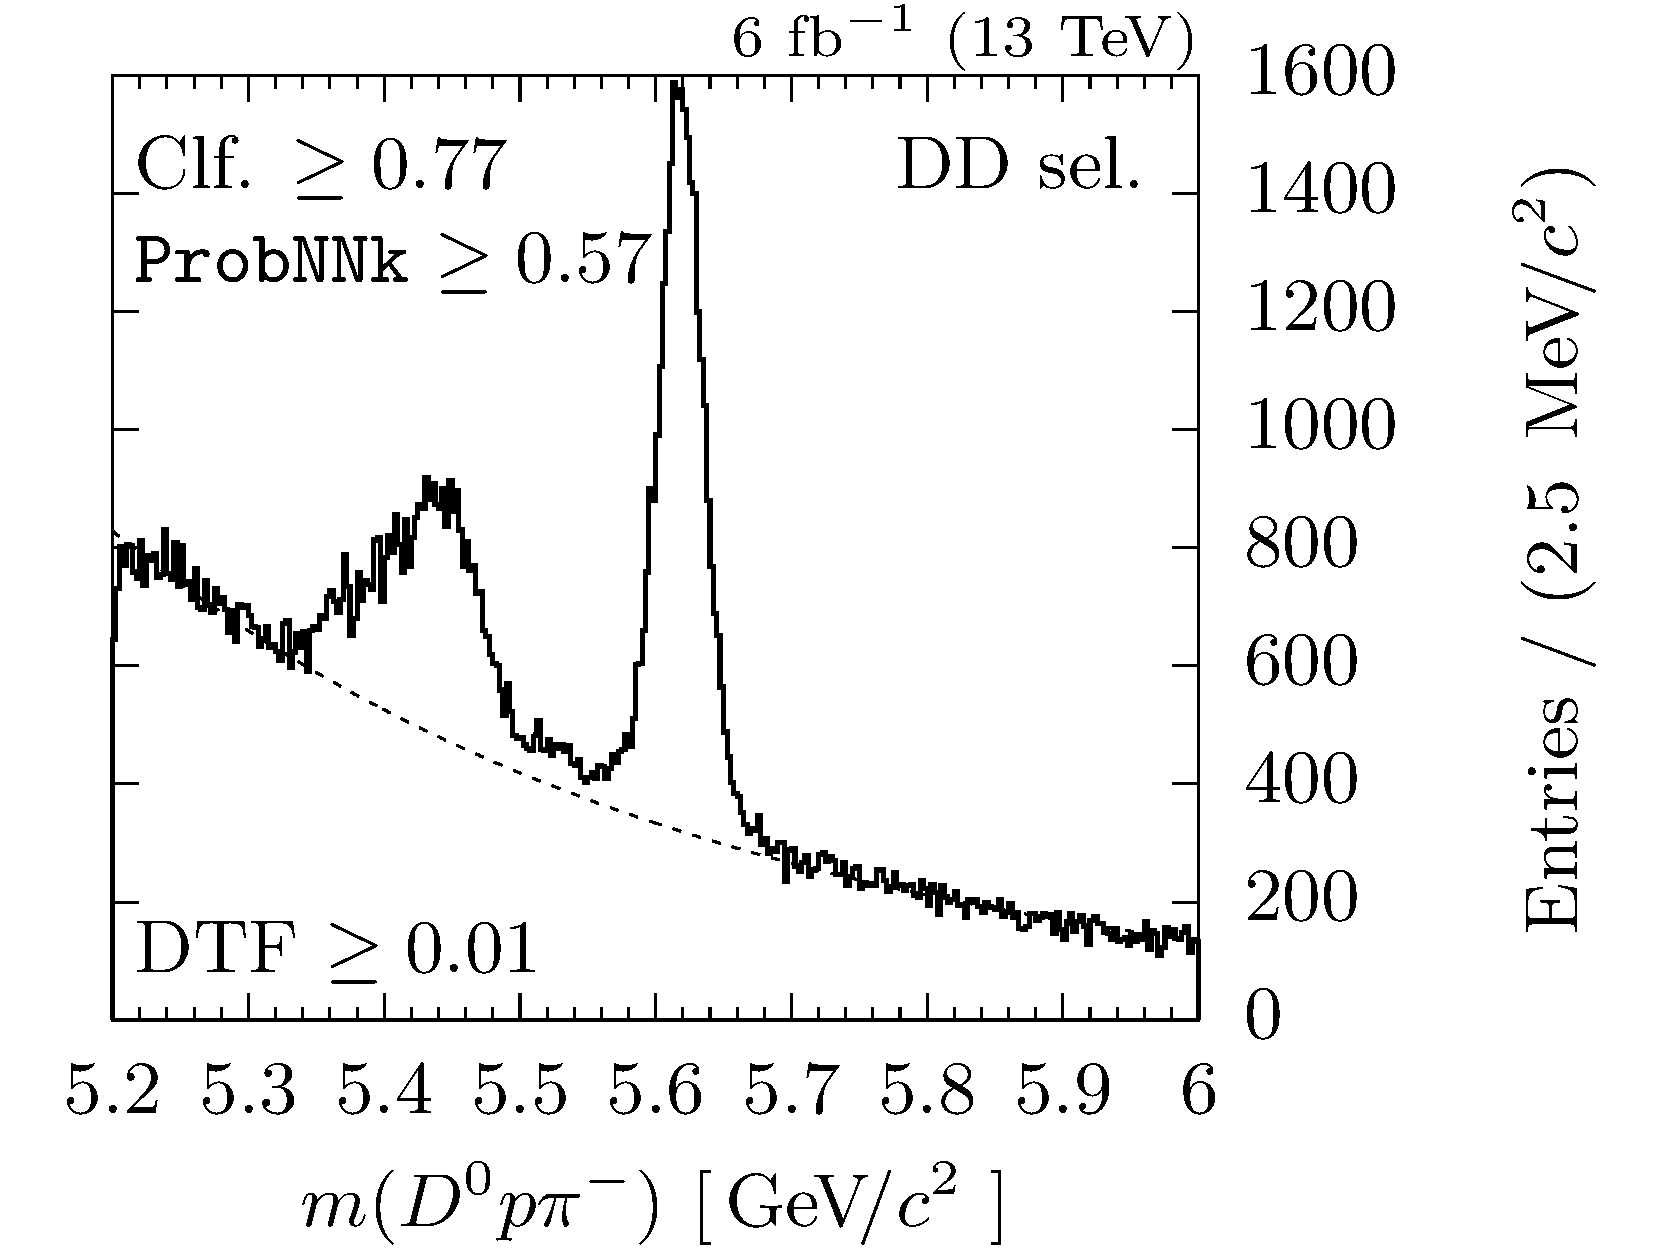
\includegraphics[scale=1.]{Lb2Dzppi_mvaxcheck/hLbM_DD_allcuts.png}
    \end{subfigure}
    \par\bigskip 
    \begin{subfigure}{.49\textwidth}
        \centering
        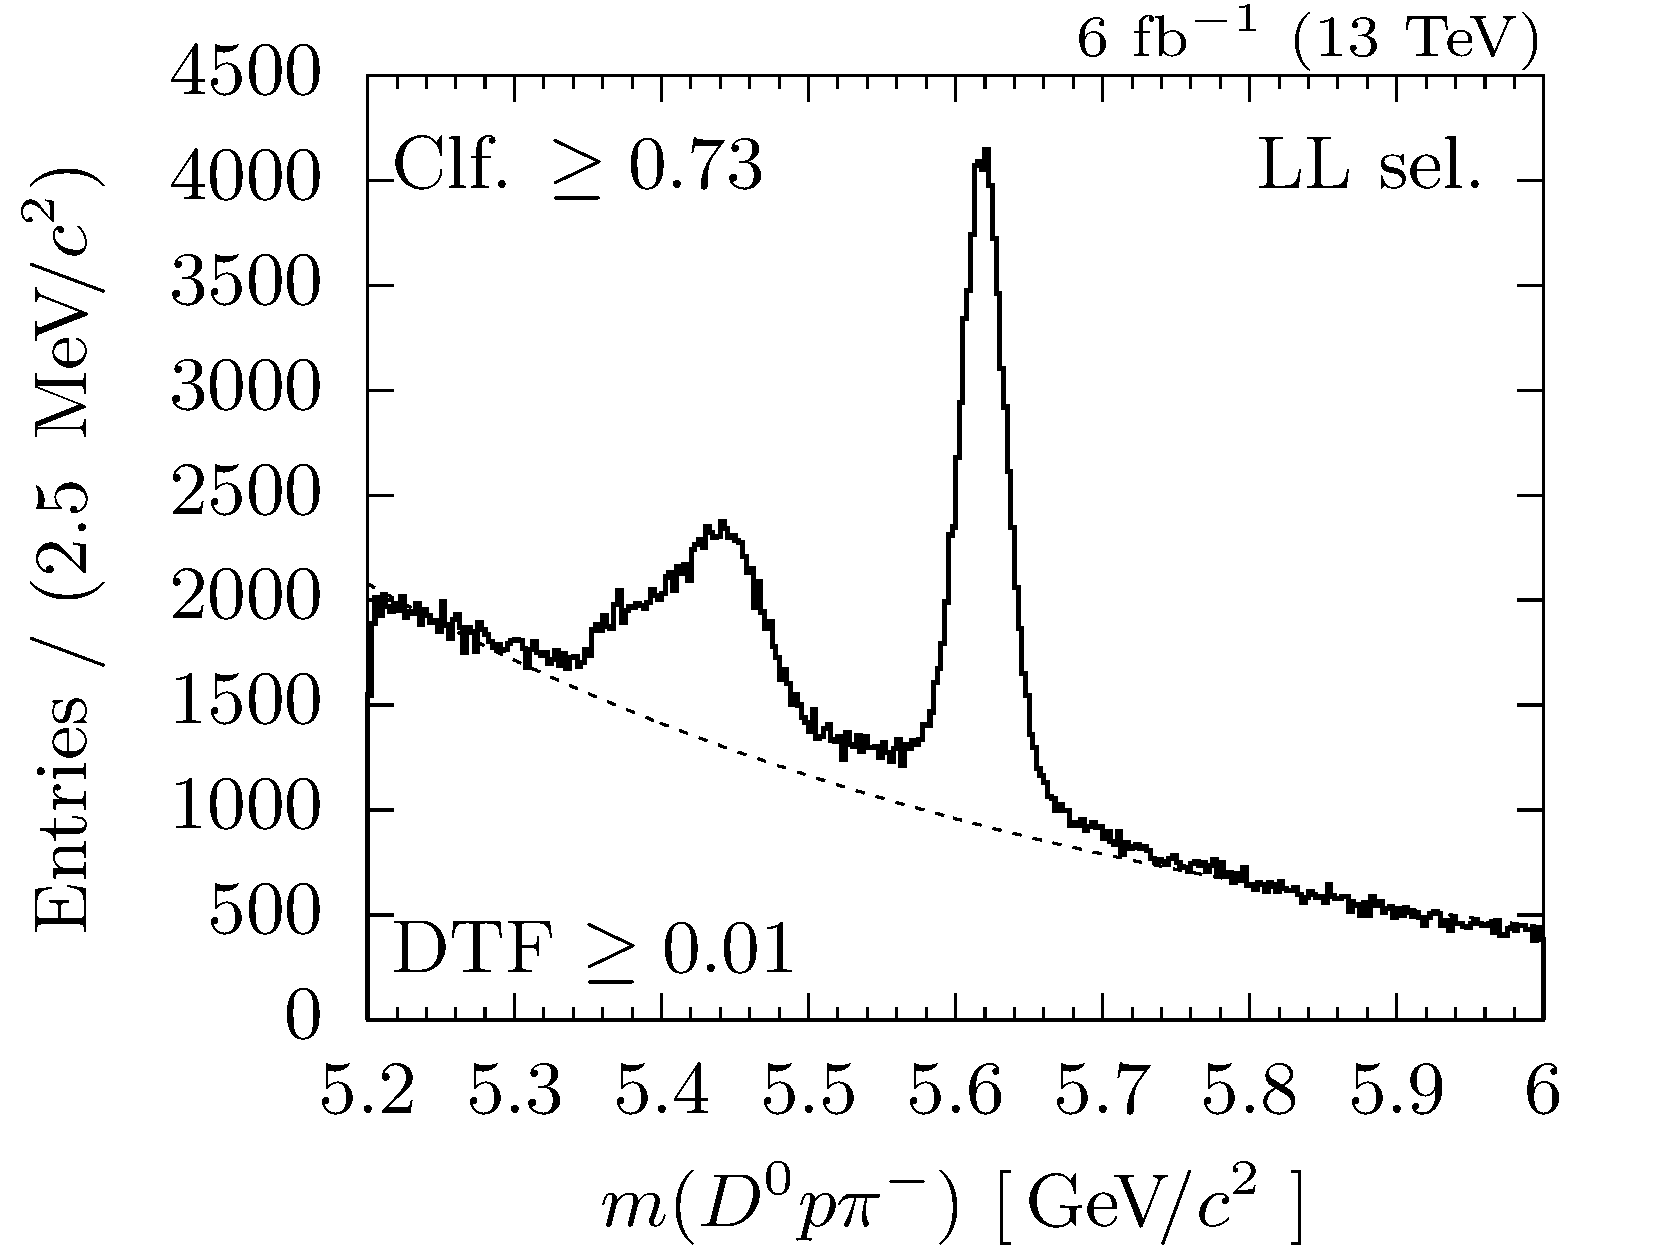
\includegraphics[scale=1.]{Lb2Dzppi_mvaxcheck/hLbM_LL_no_kProbNNk.png}
    \end{subfigure}
    \begin{subfigure}{.49\textwidth}
        \centering
        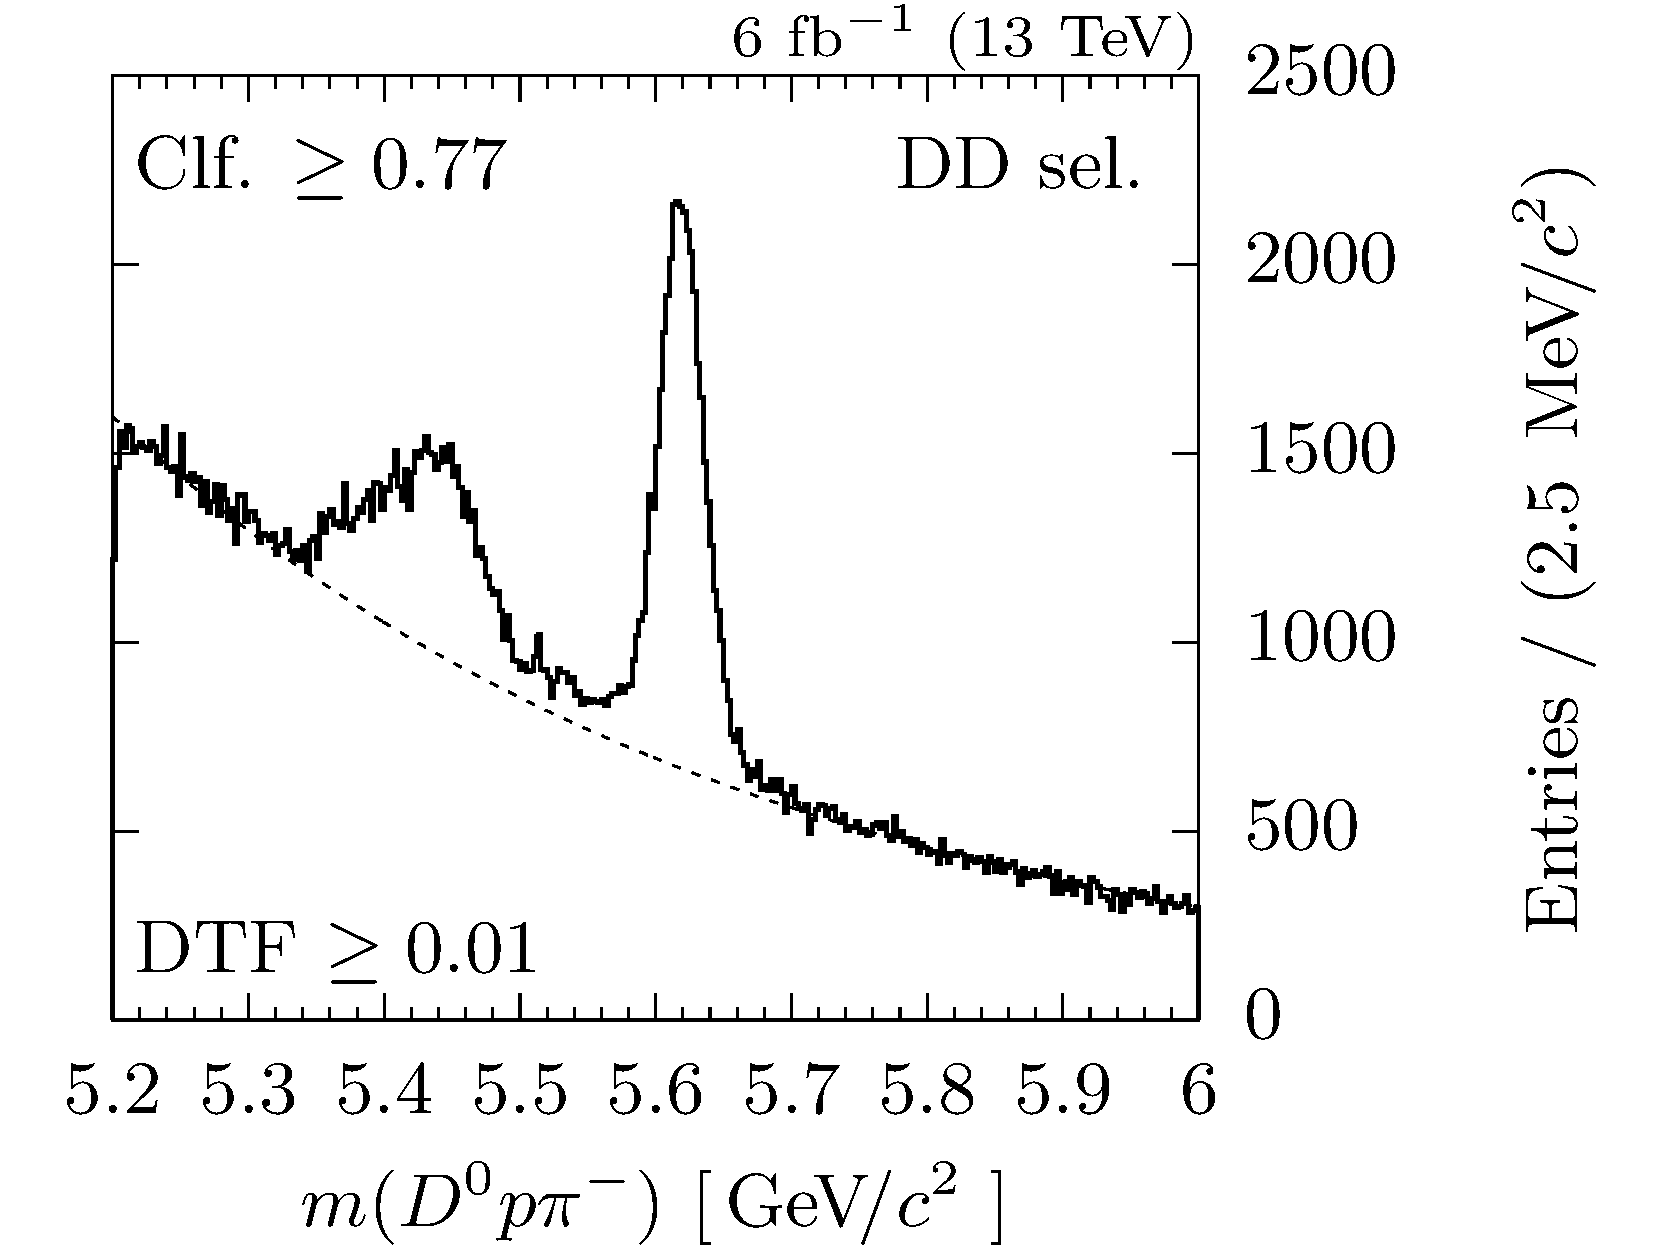
\includegraphics[scale=1.]{Lb2Dzppi_mvaxcheck/hLbM_DD_no_kProbNNk.png}
    \end{subfigure}
    \caption{Background fits to the invariant mass $m(\Dz\proton\pim)$ used for extracting the signal yield of \decay{\Lb}{\Dz\proton\pim} decays. The abbreviations \textit{LL sel.} and \textit{DD sel.} refer to the choice of thresholds which obey the dedicated \decay{\Lb}{\Dz\Lz} tight selection for \gls{LL} and \gls{DD} tracks, respectively. The yields are used to estimate the efficiency of the \texttt{ProbNNk} classifier by taking the ratio of the fitted yields $n_F$ (top) and $n_{F \setminus f}$ (bottom).}
    \label{fig:LbToDzppi_mvaxcheck_hLbM}
\end{figure}

\begin{figure}[htbp]
    \centering
    \begin{subfigure}{.49\textwidth}
        \centering
        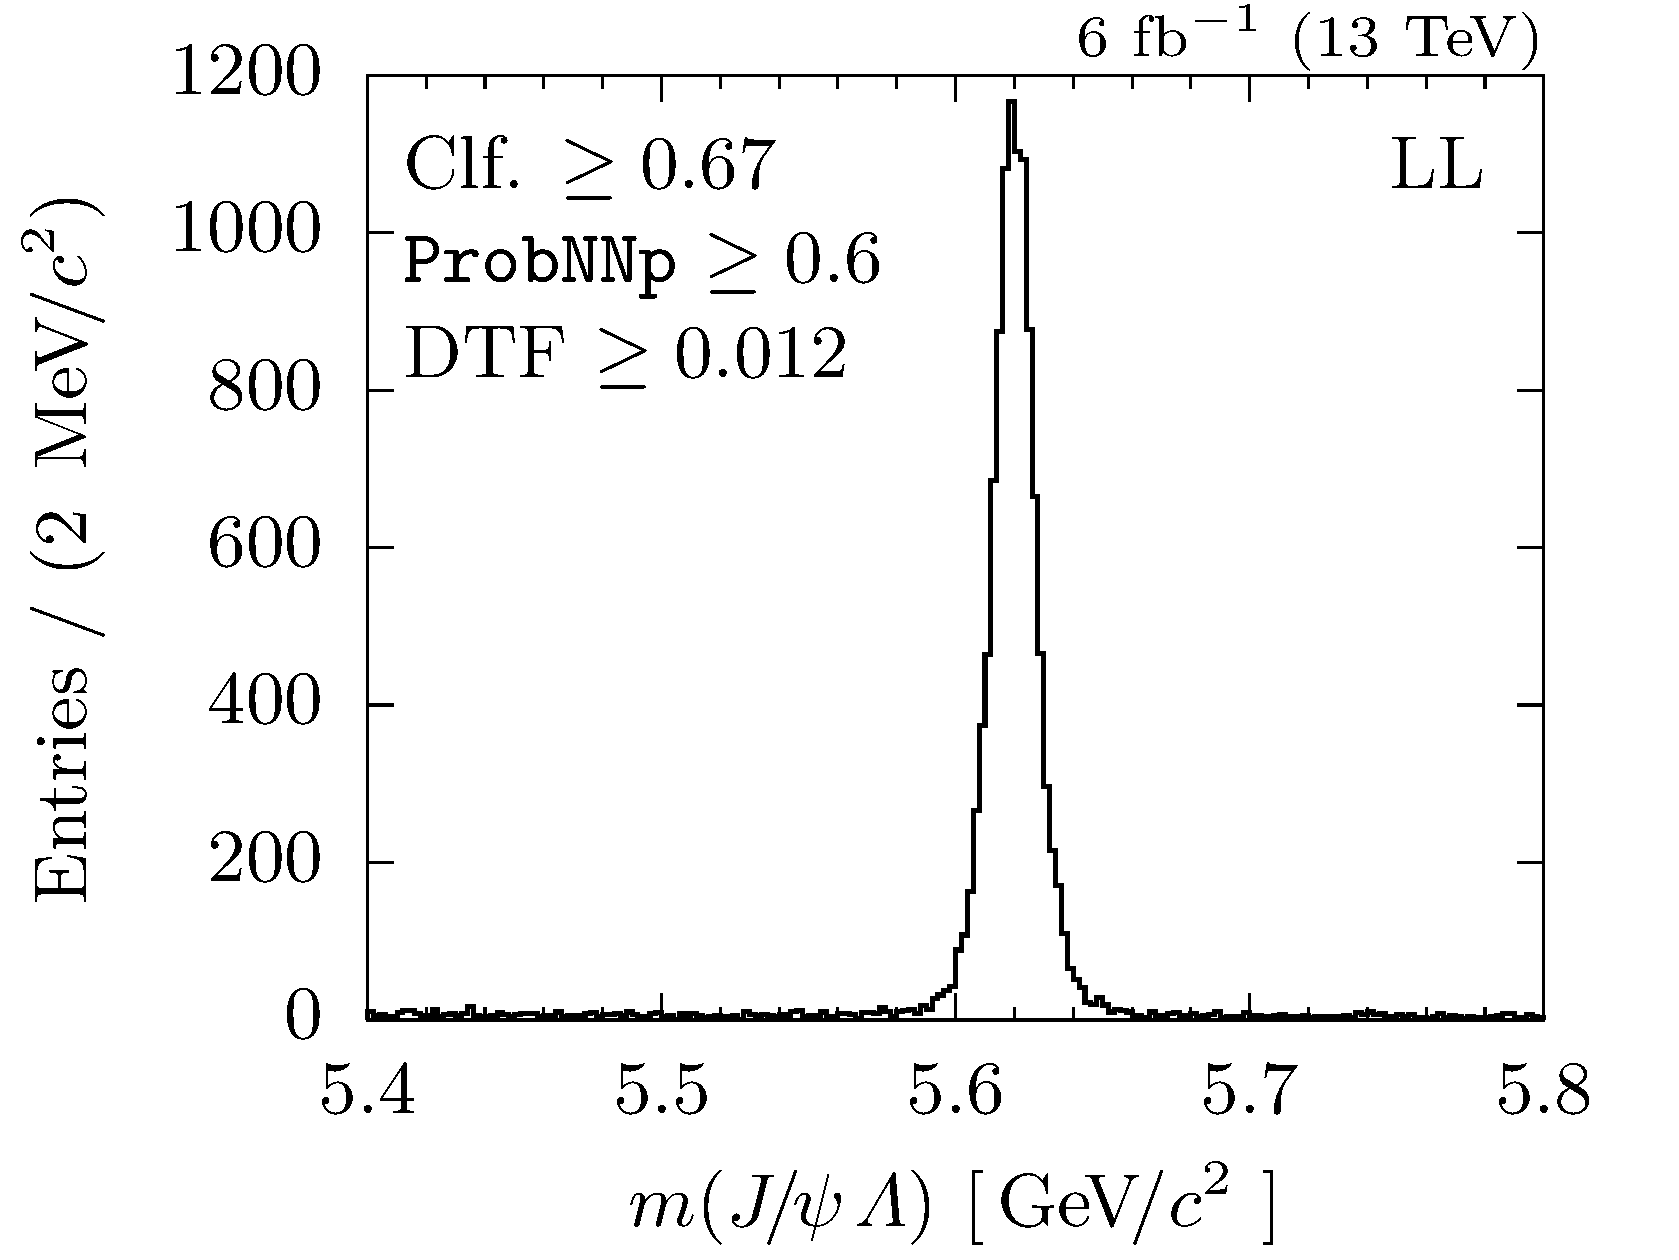
\includegraphics[scale=1.]{Lb2JpsiLz_mvaxcheck/hLbM_dtf_LL.png}
    \end{subfigure}
    \begin{subfigure}{.49\textwidth}
        \centering
        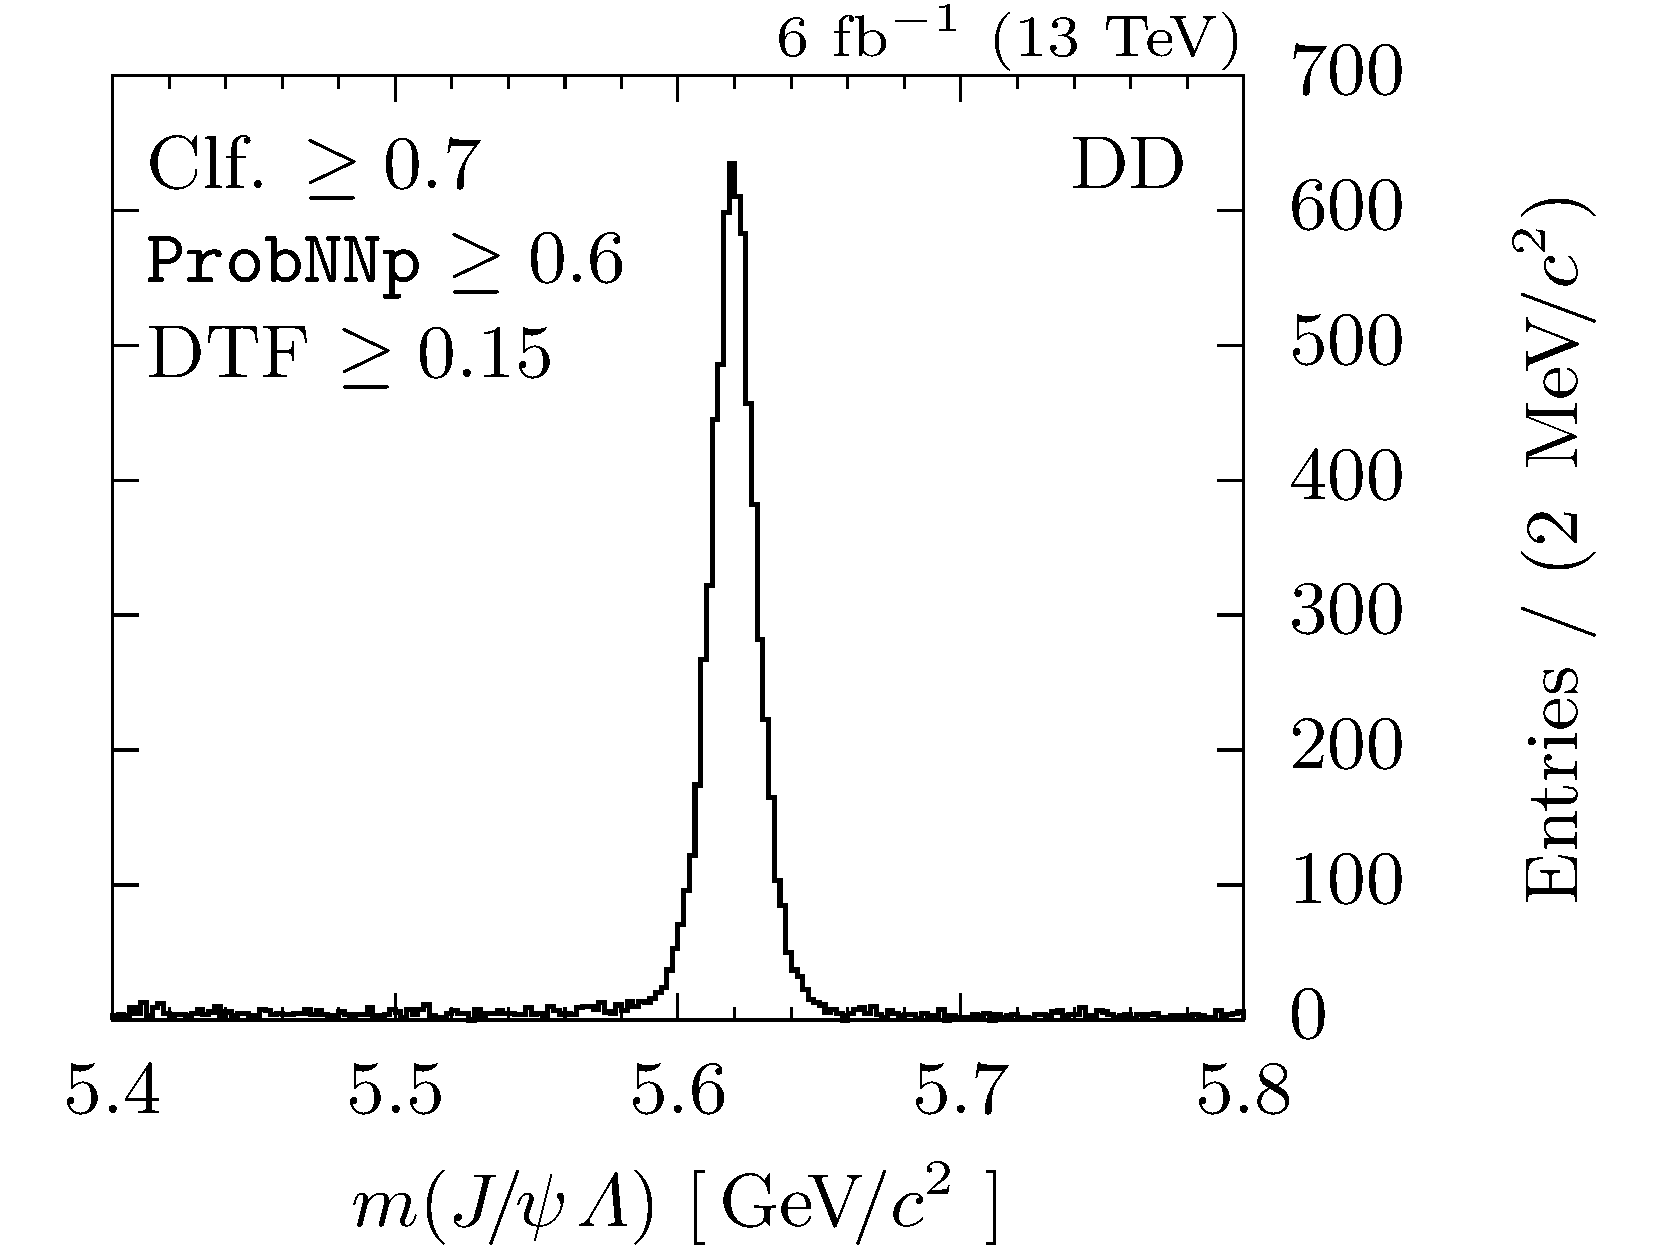
\includegraphics[scale=1.]{Lb2JpsiLz_mvaxcheck/hLbM_dtf_DD.png}
    \end{subfigure}
    \caption{Invariant mass distribution of \jpsi and \Lz candidates, refined via a \gls{dtf}, as used for estimating $n_F$ (\decay{\Lb}{\jpsi\Lz} proxy mode).}
    \label{fig:LbToJpsiLz_mvaxcheck_hLbM_allcuts}
\end{figure}

Deviations from one in the ratios of $\varepsilon_f$ of recorded data and simulated events are considered as systematic uncertainties due to fidelity issues of simulated events.
The sum in quadrature of the residuals (as listed in Tab.~\ref{tab:apdx_mva_xcheck_effs}) is used as a conservative approximation of the overall uncertainty.

\section{Fidelity of the DTF Probability Distribution}
\label{sec:apdx_mva_xcheck_pdtf}
Splitting our handcrafted classifier into two parts, \ie{}, the \Lz and \Lb-\Dz classifier, leverages the outlined cross checking of the estimated efficiency in the proxy modes \decay{\Lb}{\jpsi\Lz} and \decay{\Lb}{\Dz\proton\pim}, respectively.
This assumption of similar distributions among our primary mode \decay{\Lb}{\Dz\Lz} and the proxy modes does not hold for the $\chi_\text{DTF}^2$ distribution of the \gls{dtf} if they are not genuinely $\chi^2$-distributed with the correct \gls{dof}.\footnote{If $\chi^2$ distributed with the correct \gls{dof} the distributions transform under Eq.~\eqref{eq:fitprob} to uniform distributions and are thus equal.}
On the one hand, the \gls{dtf} probability is not uniformly distributed as discussed in Appx.~\ref{chap:apdx_fitprob}.
On the other hand we have no other way to cross-check the efficiency of the \gls{dtf} probability and therefore will stick to this approach anyhow and consider the results as approximations.

As listed in Tab.~\ref{tab:apdx_mva_xcheck_effs} we determined $\varepsilon_f$ for the \gls{dtf} probability in both proxy modes where we took the thresholds of the dedicated \decay{\Lb}{\Dz\Lz} tight selection for the \decay{\Lb}{\jpsi\Lz} proxy and $0.01$ for the \decay{\Lb}{\Dz\proton\pim} proxy.
The choice of the latter is rooted in a correlation between the \gls{dtf} probability and the bias of the respective fit model.
We consider this a minor issue due to redundancies in the \decay{\Lb}{\jpsi\Lz} mode.
Further, we find that the large deviation for \gls{DD} tracks dominantly is caused by large $\chi_\text{DTF}^2$ values (see below) and thus would likely have shown up also for this lowered threshold, if present.

In Fig.~\ref{fig:apdx_mva_xcheck_hLbM_DD_no_pdtf_fit} we show the fit that we used to extract $n_{F \setminus f}$ for the \gls{dtf} probability (\gls{DD} tracks).
Regarding the logarithmic $y$-axis we exclude that the deviation is introduced by a bias of the fit model.
In Fig.~\ref{fig:apdx_mva_xcheck_cdf_pdtf} we show the cumulative distribution of the \gls{dtf} probabilities for \gls{LL} and \gls{DD} tracks.
We see that the deviation for \gls{DD} tracks comes from an initial offset at large $\chi_\text{DTF}^2$ values and then keeps this difference.
Based on this we conclude that this effect has to be attributed to the \Lz baryon itself, due to the good agreement for \gls{LL} tracks in both proxy modes.
Since daughters of track type \gls{DD} of the \Lz baryons are the only particles in our consideration whose momentum information is not taken from the \gls{velo} (by definition), this issue is likely to be rooted in an incomplete error matrix for \gls{DD} tracks.
Correcting this error matrix is out of scope of the present analysis and we will therefore take the full deviation as an systematic uncertainty.

\begin{figure}[htbp]
    \centering
    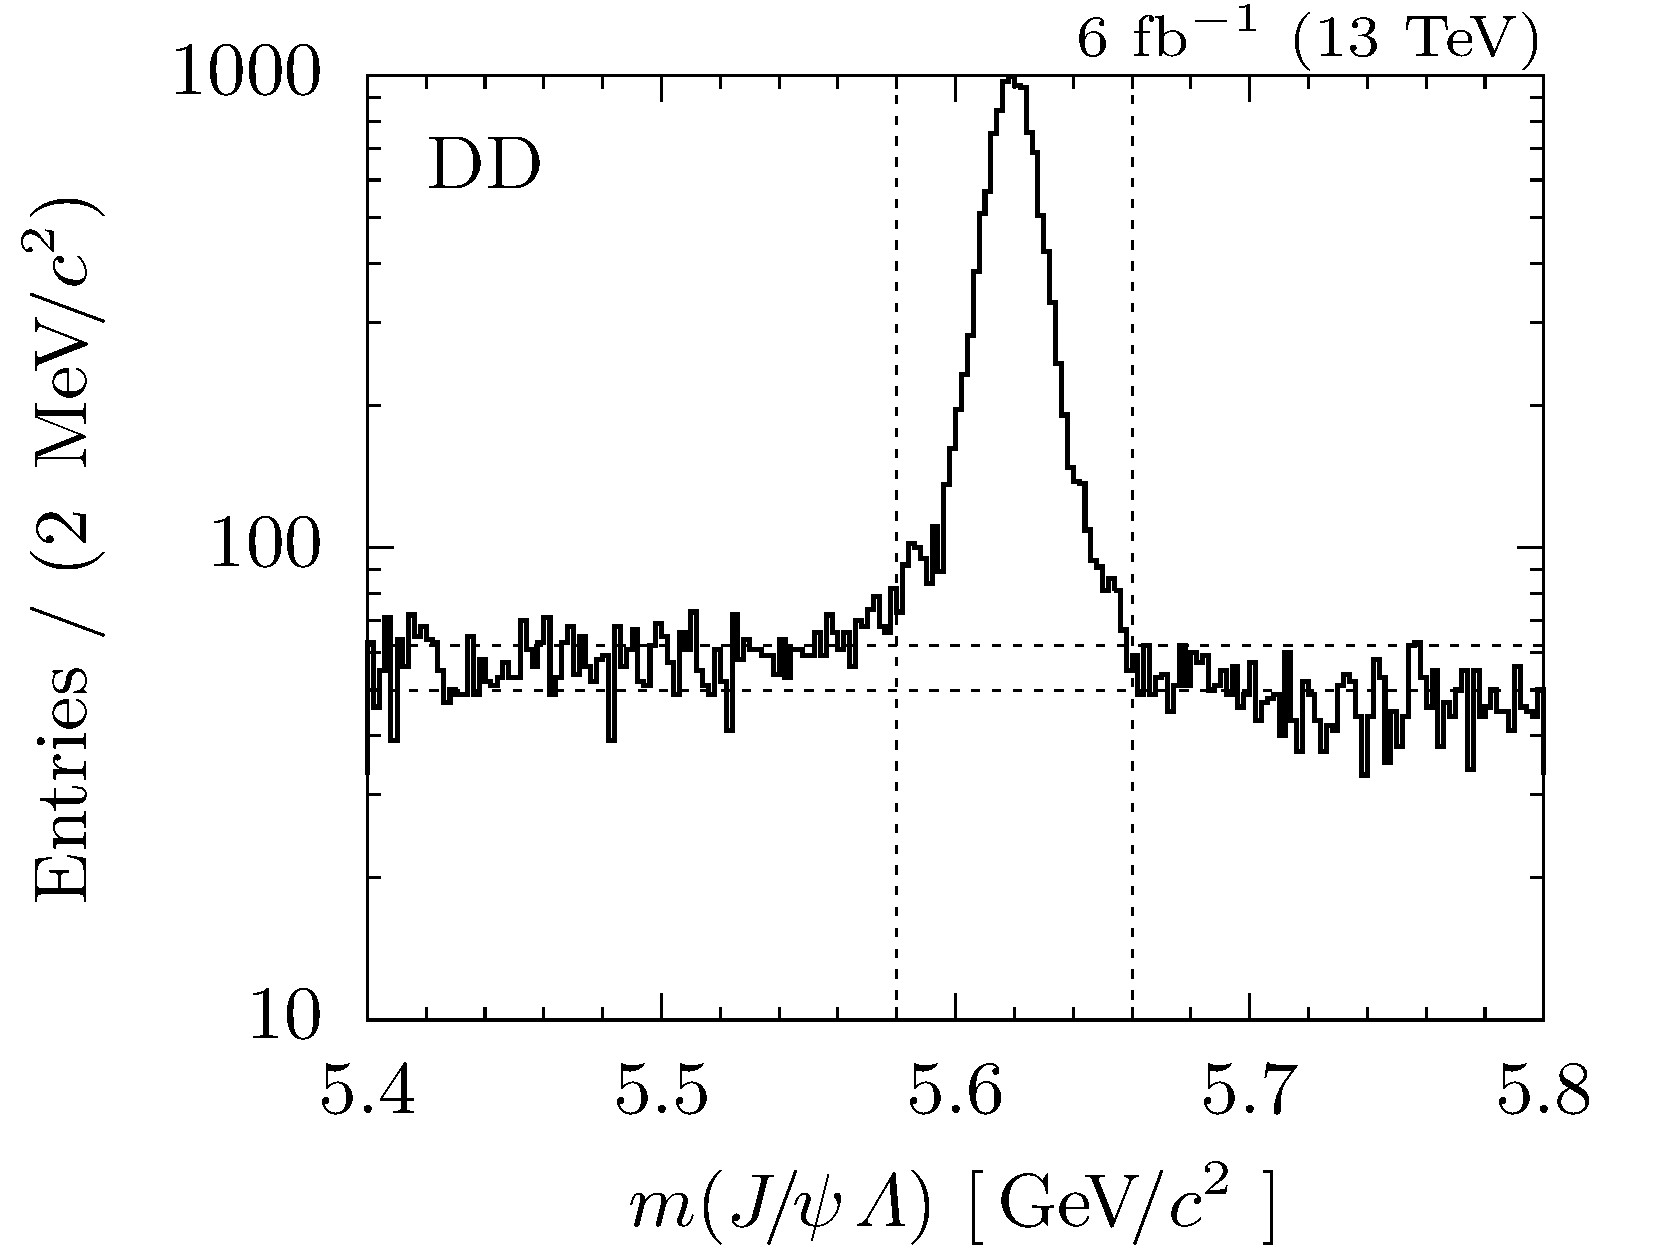
\includegraphics[scale=1.]{Lb2JpsiLz_mvaxcheck/hLbM_dtf_DD_no_pdtf_fit.png}
    \caption{Combined invariant mass of \jpsi and \Lz candidates used to extract the signal yield $n_{F \setminus f}$ for the \gls{dtf} probability (\gls{DD} tracks) via sideband subtraction. The sideband subtraction is evaluated twice, once using only the lower sideband, and a second time using only the upper sideband. The difference between both evaluations is taken as a systematic uncertainty. We note that regarding the large signal to background ratio, biases of the fitting technique affect the numerical value of the yield only slightly.}
    \label{fig:apdx_mva_xcheck_hLbM_DD_no_pdtf_fit}
\end{figure}

\begin{figure}[htbp]
    \centering
    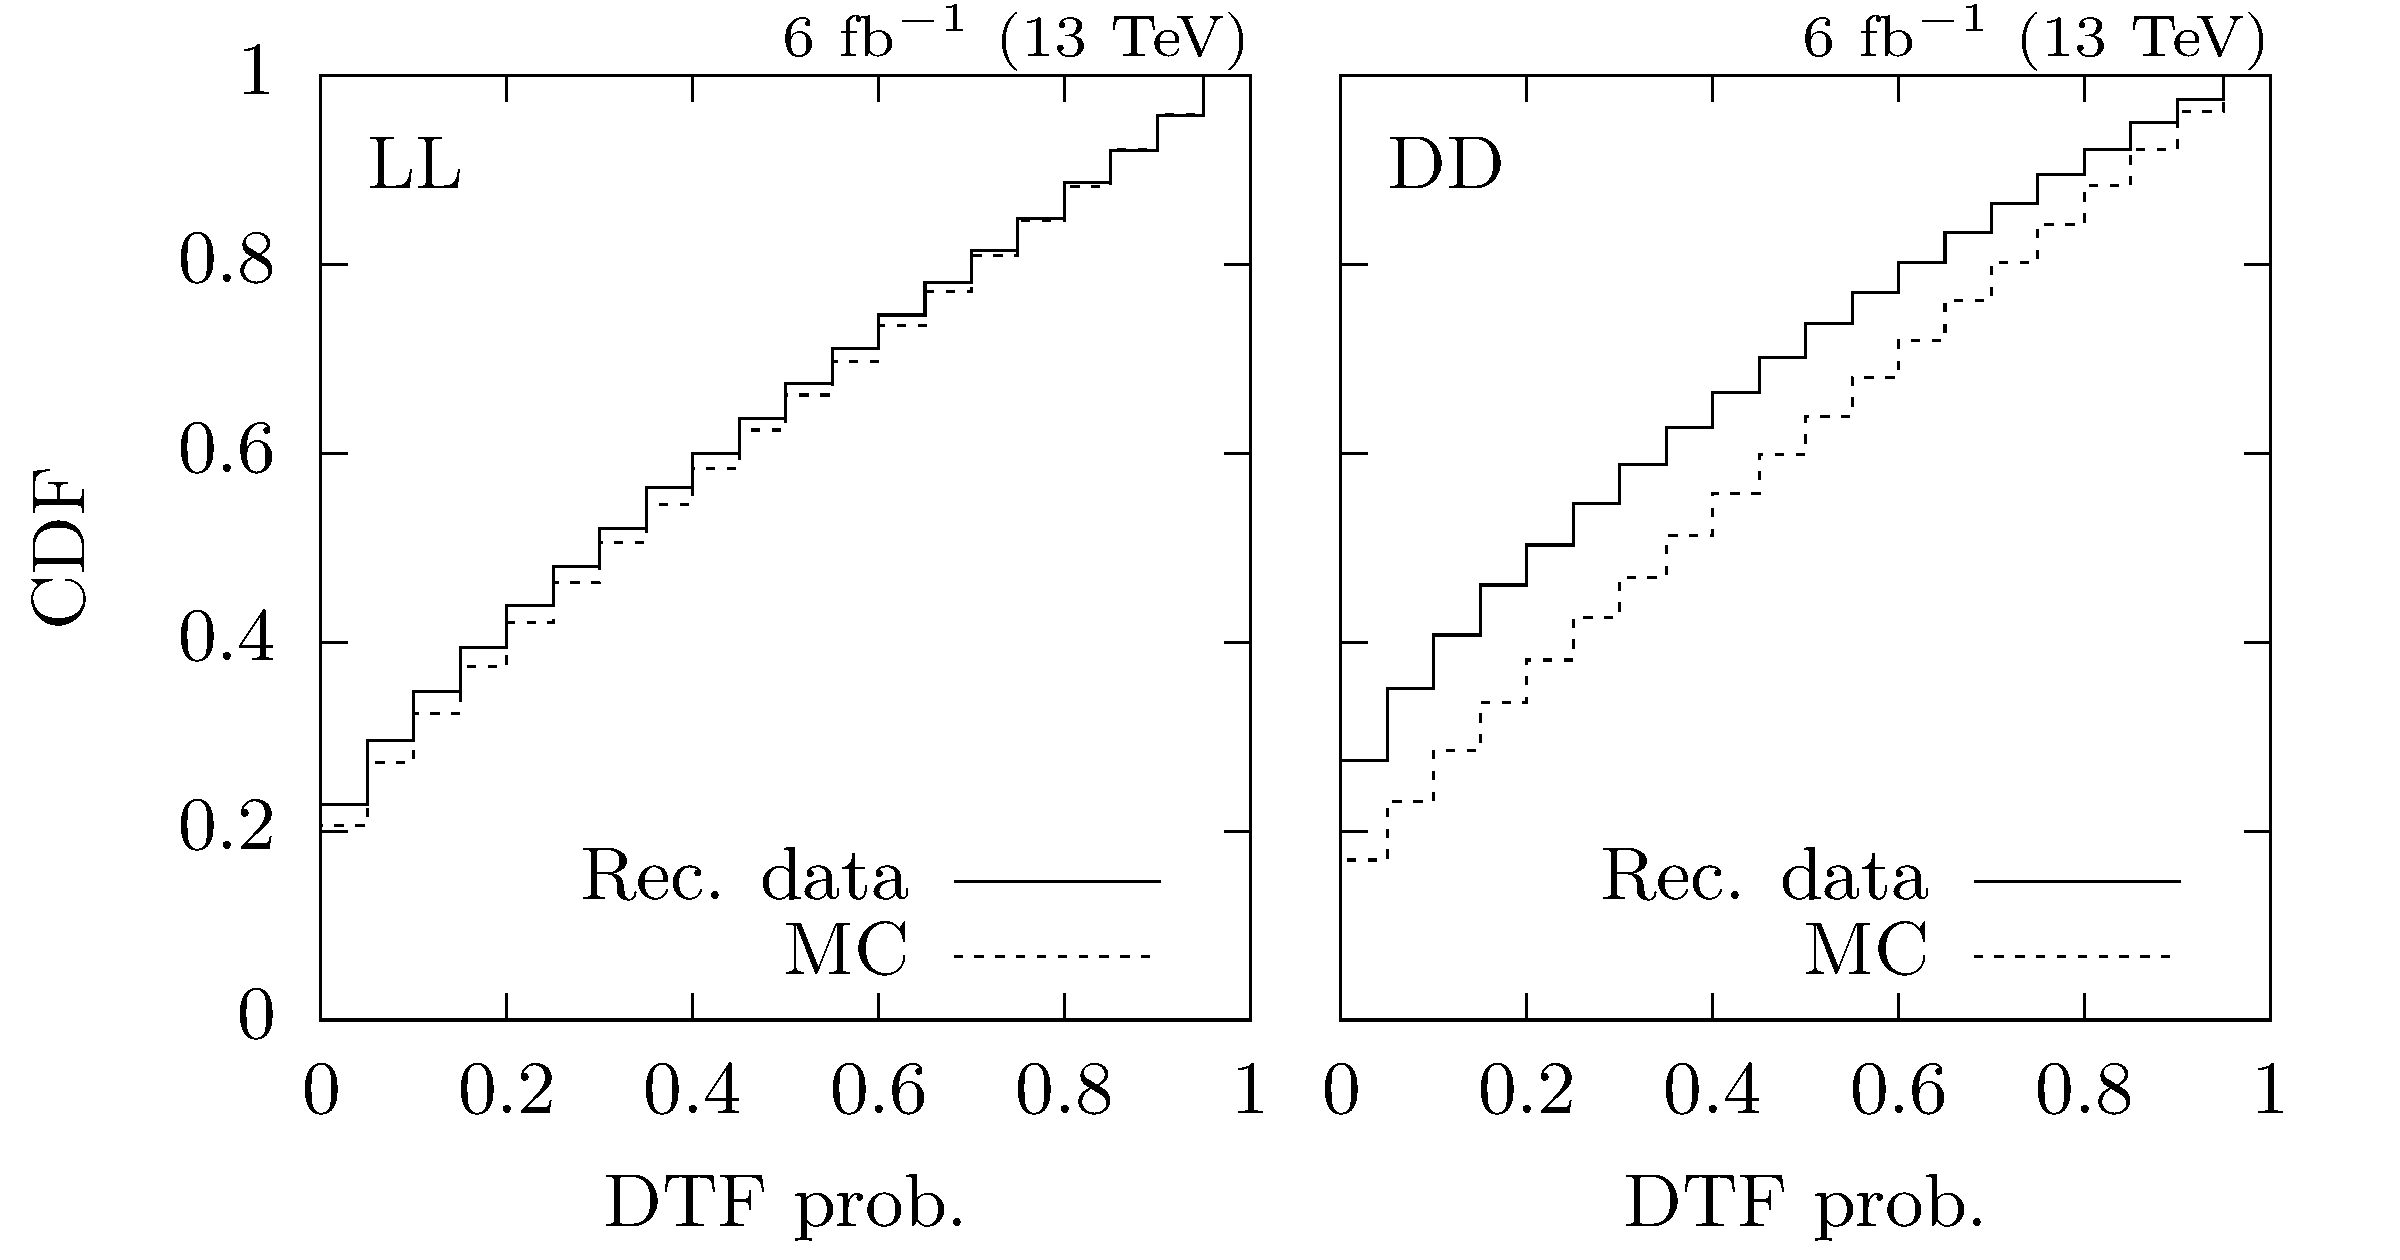
\includegraphics[scale=1.]{Lb2JpsiLz_mvaxcheck/cdf_pdtf.png}
    \caption{Cumulative distribution function (CDF) of the \gls{dtf} probability distributions for \gls{LL} and \gls{DD} tracks. The CDFs are extracted via sideband subtraction and are thus binned. The solid and dashed line refer to recorded data and simulated events, respectively. The $y$-value of a bin with high-edge $x$ thus corresponds to the sum of all events with \gls{dtf} probability $\le x$. In particular, the first bin includes the effects of $\chi_\text{DTF}^2$ cut-offs at large values.}
    \label{fig:apdx_mva_xcheck_cdf_pdtf}
\end{figure}
